\chapter{绪论}
\label{chap:introduction}

\section{研究背景与意义}
软岩是地球表面分布最为广泛的一种岩石,我国软岩分布范围很广,在云贵高原、湘浏盆地、四川盆地、甘肃东北部、东南沿海和东北地区都有软岩成片或零星分布\cite{黄志全2021}。
%它是一种特定环境下的具有显著塑性变形的复杂岩石力学介质。根据软岩特性的差异及产生显著塑性变形的机理,软岩可分为4大类,即膨胀性软岩、高应力软岩、节理化软岩和复合型软岩。
%近年来,建筑工程领域的学者对软弱围岩的理论和应用进行了更深一步的研究,但软岩的界定在科学界尚未得到统一的认识,大体上分为定性描述和定量指标两种。

%定性描述认为软岩是松散、破碎、软弱、强风化以及膨胀性一类岩石的总称。定量指标则是以岩石单轴抗压强度值作为评判依据,国际岩石力学学会(International Society for Rock Meehanies, ISRM)定义软岩为单轴抗压强度在\SIrange[]{0.5}{25}{MPa}的一类岩石。在我国,依据《岩土工程勘察规范》(GB 50021—2009)、《铁路工程地质勘察规范》(TB10012-2007)等规范,对岩石的具体分类如下表~\ref{tab:岩石坚硬程度划分}。

%\begin{table}[h]\small
%	\centering
%	\caption{岩石坚硬程度划分}
%	\begin{tabular}{c|c|c|c|c|c|c}
%		\hline
%		\multirow{2}{*}{岩石类别}    & \multicolumn{2}{c|}{硬质岩} & \multicolumn{3}{c}{软质岩}             \\ \cline{2-6} 
%		& 坚硬岩        & 中硬岩        & 较软岩 &软岩 & \multicolumn{1}{c}{极软岩} \\ \hline
%		\multicolumn{1}{c|}{饱和单轴抗压强度$R_c$(MPa)} &   
%		${R_c}$ $\textgreater$ 60     & 30 $\textless$ ${R_c}$ $\leq$ 60             & 15 $\textless$ ${R_c}$ $\leq$ 30   & 
%		5 $\textless$ ${R_c}$ $\leq 15$
%		& \multicolumn{1}{c}{${R_c}$ $\leq$ 5}    \\ 
%		\hline
%	\end{tabular}
%	\label{tab:岩石坚硬程度划分}
%\end{table}

随着我国基础建设的加速推进,水力资源的大规模开发,铁路、公路交通的迅速拓展,以及深部矿产资源的开采等,这些工程均面临着在软弱岩体中进行地下开挖的的问题。这些工程的稳定性问题总会受到各种因素的影响。
例如,盘道岭隧洞施工期及建成后,二次衬砌混凝土产生了大量的裂缝,研究发现,裂缝的主要原因是由于早期收敛值小于规范值较多,后续取消系统锚杆导致发生大量流变变形\cite{陈晓东1996}。
小浪底水利枢纽孟溪灌区总干渠7号隧洞在施工过程中出现裂缝、下沉、底板拱起等现象,经分析和结构应力计算,认为是地质情况的变化导致衬砌受力恶化,原衬砌厚度不足,侧墙和底板实际应力大于规范允许值\cite{黄晓林2008}。
小康矿S2S2工作面运输巷纳巷道发生变形破坏、顶板严重流变、底鼓量大 、支护构件发生屈服破断,整体工程存在道围岩破碎、变形大、支护困难等问题\cite{王国强2018}。
针对郑州粉土基坑开挖对下卧地铁隧道的影响的研究表明,使用常规分层开挖的方法对隧道竖向最大位移值超过了郑州地铁保护标准\cite{郭院成2019}。

由上述这些案例可以发现,地下开挖工程中围压大都会发生较大变形,而无论是由于施工方法或地质条件变化导致的长期变形增大一般都会产生裂缝甚至出现垮塌的工程问题。
分析原因认为其诱发原因可能与长期流变变形有关,流变变形会导致地下工程的整体变形远大于预期。
在软弱岩体中进行地下工程开挖,需要关注的一个重要问题就是如何解决施工过程中的安全和后期运行中的岩体流变问题。无论是地面的边坡、路基、水电大坝工程,还是地下洞室、隧道、能源储库等岩石体工程,均会出现不同程度的流变现象。在地下洞室和巷道开挖中,流变通常不会在刚开挖完就发生失稳破坏,但可能会在长期建设或后期运营中,随着时间的推移其内部不断演化,岩体呈现出显著的流变特性,甚至发生坍塌,这对工程建设的稳定与安全有着重大隐患。因此软岩中的流变问题应该受到关注。

再加之,目前工程取向于深部化,深部工程与浅层施工的明显区别在于,深部岩石所处的“三高一扰动”的特殊环境。“三高”指的是高地应力、高地温、高渗透压,“一扰动”主要是指强烈的开采扰动\cite{深部岩体力学基础}。
其中高温是引起深部岩石力学性质变化的重要因素。根据量测,越往地下深处,环境温度越高,地热梯度一般为\SIrange[]{30}{50}{\celsius /km}。岩石在超出常温的环境下,表现出的力学性质和变形特性与普通环境条件下有和大差别,深部岩石在蠕变时易受到高温环境的影响更易发生损伤变形,高温会导致岩石的晶体结构发生变化,而晶体结构的变化会导致基本物理力学性质的变化\cite{Roland1988},进而岩石短期强度及长期强度与常温相比均会发生很大变化。岩石在经历高温作用后,其强度(包括单轴抗压强度、抗拉强度)、波速(包括压缩波波速和剪切波波速)、弹性模量都会降低,孔隙度增大。

综上所述,面临工程深部化,对于诸多的软弱围岩的地下工程开挖稳定性需要关注,我们可以从力学角度对软岩的流变过程进行分析,而深部软岩受到特殊的高温环境的影响,因此需要对软岩的热力耦合特性进行研究。

%通过较为系统的理论分析、试验研究以及数值模拟等手段对工程岩体的流变特性进行研究,建立其泥岩的流变本构模型,并结合工程实例,对隧道围岩的长期稳定性进行分析。该研究一方面可用于指导和优化工程的设计与施工,对确保工程施工安全及其长期稳定具有重要的意义;另一方面,该研究可丰富类似岩体条件下地下工程的研究理论和方法,为后续类似工程问题的研究提供一定的参考。

\section{国内外研究现状}

岩石流变,是工程界和学术界共同关心的问题。岩石流变是指随着时间的推移,岩体呈现出的蠕变、应力松弛以及强度的时间效应等特性。在过去的几十年里,岩石的弹塑性和蠕变分析一直是国内外学者主要讨论焦点。
孙钧(2007)对于岩石流变力学及其工程应用的讨论为我们介绍了国内外岩石流变问题的研究进展\cite{孙钧2007},对岩石流变的问题,从微观机理、室内外试验到本构模型及参数拟合,均有人开展了广泛的研究工作,分类总结研究现状如下:


%\subsection{岩石流变机理的研究}

%在岩石流变的过程中,受到外界因素,如温度、应力、含水率等等,都会影响其流变过程。
%邵珠山等(2018)引入了温度变化对岩石变形特征的影响,基于Burgers流变模型,推导出了变温度场作用下的岩石流变方程,研究结果表明,由于温度变化产生的热应力会加速岩石试样的损伤,在减速蠕变和稳定阶段,变温场下的应变速率和应变量均显著增加\cite{邵珠山2018}。
%Maranini等对石灰岩采样进行了单轴、三轴压缩蠕变试验,指出了该类石灰岩的流变细观变形机理:低围压条件下裂隙的扩展,高应力条件下孔隙的塌陷\cite{Maranini1999}。

%另外,有些学者们希望通过微观上对岩石的晶体结构进行研究,探究岩石流变过程的本质。通过对脆性岩石的蠕变特性研究,Scholz CH认为脆性岩石的蠕变现象主要是岩石基于时间效应的微破裂过程\cite{Scholz.C}。
%Roland Pusch指出岩石发生蠕变的物理机理是由于沿着晶格面以及沿着接触的、胶结的或非胶结的晶体之间的界面出现了剪切位移的缘故,并基于统计力学原理提出了岩石蠕变作为随机过程的数学表达式\cite{Roland1988}。
%Gui Liu等在高温高压条件下对片理化花岗质糜棱岩进行了一系列流变实验,力学微观结构数据表明组构对岩石强度有显著影响,但对脆塑性转变和变形机制几乎没有影响\cite{Liu2017}。

%机理到底是什么?是否仍存在争议。

%\subsection{软岩三轴压缩力学特性试验研究}
%对于常规试验,我们通常采用单轴和三轴压缩的方式测得岩石的轴向、环向应力应变及位移,借此研究其力学特性,这也是研究岩石各项性能包括流变的基础。因此,关于软岩常规三轴试验方面的研究成果繁多。对于不同应力状态下对软岩的力学特性及变形的影响,

%李海波、陈蔚等国内外学者相继对软岩在载荷作用下的强度及变形特征与应变之间的关系进行了研究\cite{李海波2004,陈蔚2020}。
%王国民(2000)通过对软质粉砂岩进行单轴、三轴压缩试验,探究了其在三维应力下的变形和强度特征\cite{王国民2000}。
%封志军等(2005)对不同围压下红层软岩三轴应力一应变全过程进行试验,研究得到了几种典型红层软岩的抗剪强度、参与抗剪强度以及水对这两种强度的影响\cite{封志军2005}。
%杨永杰等(2006)通过对煤岩的常规三轴试验发现煤样三轴压缩强度与围压之间呈线性关系\cite{杨永杰2006}。
%曾玲玲等(2009)对软土在不同应力路径下的力学特性进行分析\cite{曾玲玲2009}。
%李翻翻等(2020)基于塑性损伤对黏土岩的力学特性与应力状态之间的关系进行研究\cite{李翻翻2020}。

%岩石在温度条件的变化下,其强度及变形特性也会受到相当程度的影响。但是,目前关于温度对岩石性质的影响研究大多侧重于如大理石、花岗岩、盐岩等具有脆性特性的硬岩上,例如刘泉声、许锡昌等(2000)初步探究了花岗岩在单轴压缩状态下主要力学参数随温度的变化规律\cite{许锡昌2000};X.L. Xu等(2018)基于Weibull分布和Lemaitre应变等效原理,建立了花岗岩热-力学耦合损伤模型框架,模拟高温高压条件下岩石的变形和破坏过程\cite{Xu2018},对于软岩相关的温度方面的研究相对较少。

%这一段需要重新考虑一下

\subsection{软岩流变试验研究现状}
在国外,岩石流变力学特性试验研究可以追溯到20世纪30年代末,Griggs(1939)最先对灰岩、页岩和粉砂岩等类软弱岩石进行了蠕变试验,指出砂岩和粉砂岩等中等强度岩石,仅当加载达到破坏荷载的\SIrange[]{1.25}{80}{\%}时,就发生了一定程度的蠕变\cite{Griggs1939}。
Paul Le Comte(1965)对人工多晶岩盐试样和单晶岩盐试样进行了蠕变试验,研究发现温度或应力差的增加会大大增加蠕变速率。围压或晶粒尺寸的增大会使蠕变速率有所降低\cite{Pual1965}。
K.A.Balthasar等(1987)研制了一种单轴应力松弛试验装置用于在实验室中研究应力松弛现象。将现场试验结果与室内试验结果进行了比较\cite{Balthasar1987}。
Haupt(1991)也对盐岩的松弛变形进行了研究,指出在整个应力松弛过程中,其岩石内部的细观结构仍保持不变,而应力松弛则在另一侧面反映了盐岩内部组构受力后的黏性效应\cite{Haupt1991}。
Maranini(1999)等对石灰岩采样进行了单轴、三轴压缩蠕变试验,指出了该类石灰岩的蠕变微观变形机理:低围压条件下裂隙的扩展,高应力条件下孔隙的塌陷\cite{Maranini}。
Hadiseh(2018)、Moslehy(2023)等都对盐岩的蠕变力学特性进行了试验研究,研究发现蠕变应变和稳态蠕变速率随轴向应力的增大而增大,而在Moslehy的研究中,还考虑了温度对盐岩蠕变过程的影响,试验表明温度升高温度会导致累积应变增加,且瞬态应变速率会受到高温环境的影响而增加\cite{Mansouri2018,Moslehy2023}。


自20世纪50年代起,我国大型工程项目的兴建,陈宗基教授首先将流变理论引入岩石力学并提出了岩石流变的概念,之后随着我国大型工程的建设,各类岩石的流变试验得以大量开展,积累了各类岩石丰富的流变试验资料及数据。
李永盛(1995)采用伺服刚性机对粉砂岩、大理岩、红砂岩和泥岩4种不同岩性的岩石进行了单轴压缩条件下的蠕变和松弛试验,发现在一定应力作用下,岩石材料一般都出现蠕变速率减小、稳定和增大三个阶段,但各阶段的出现与持续时间和岩石的性质与围压有关\cite{李永盛1995},该研究的不足之处在于受到设备和试验环境的影响,所观察的岩石流变现象较短,流变过程需要更长时间的实验观察以得到更准确的结果。
徐平(1996)、夏熙伦(1996)等对三峡花岗岩进行了单轴蠕变试验,给出了三峡花岗岩的蠕变经验公式,认为三峡花岗岩存在一个应力门槛值$\sigma$。当应力水平低于$\sigma$时,可采用广义Kelvin模型来描述三峡花岗岩的蠕变特性;当应力水平高于$\sigma$时,采用西原模型来描述,并给出了相应的蠕变参数\cite{徐平1996,夏熙伦1996}。

近年来,软岩作为重大建(构)筑物地基的情况愈益多见,其变形大、强度低,具有更为显著的流变特性。因而研究覆盖我国广大地域的软岩的流变力学特性具有重要的工程实用价值。
赵延林(2008)、谌文武(2009)、熊诗湖(2016)、邹建超(2015)等都通过分级加载试验的方式对软岩的流变特性进行了研究,并提出了符合该软岩的蠕变特性的本构模型,并根据实验结果确定其中的参数\cite{赵延林2008,谌文武2009,熊诗湖2016,邹建超2015},不过在这些文章中基本上是以单轴分级加载的方式进行的试验,对于围压及卸荷对流变过程的影响未考虑在内。

针对这方面的问题,王红伟等(2001)针对“三软”煤层巷道围岩大变形、难支护的具体情况,以显德汪矿的主运输大巷为研究对象,进行了三轴压缩流变试验,获得泥岩的流变参数\cite{王红伟2001}。
范庆忠等(2007)等在低围压条件下对龙口矿区含油泥岩的蠕变特性进行三轴蠕变压缩试验研究,试验结果表明,含油泥岩存在一个起始蠕变应力阈值,该阈值随围压的加大呈线性增加,其蠕变破坏应力也大致与围压成比例关系\cite{范庆忠2007},
李建林等(2007)结合三峡丁程永久船闸高边坡岩体,根据其各项物理力学特性,模拟制作了部分试件,对节理岩体的加卸载应力——应变关系、卸荷岩体的各向异性、流变特性、强度准则进行试验研究\cite{李建林2007}。
左亚(2014)采用RLW—2000岩石三轴流变试验系统进行了恒轴压卸围压的流变试验,分别控制轴压与围压的变量,分析了试样轴向及侧向流变随时间的变化规律及破化形态\cite{左亚2014}。
王宇等(2015)采用 RLW 一2000 三轴流变仪对泥质粉砂岩进行三轴压缩流变试验,通过试验发现软岩加速流变阶段速率随围压升高而降低,其流变破坏仍以剪切破坏为主\cite{王宇2015}。
马冲等(2017)通过对粉砂质泥岩进行了不同围压和渗透压下的三轴蠕变实验,探讨了围压和渗透压对岩体蠕变
特性的影响过程和机理。采用等时应力—应变曲线法和稳态蠕变速率法求得了粉砂质泥岩在不同围压和渗透压下的蠕变长期强度\cite{马冲2017}。
胡华等(2019)选取软弱砂岩为研究对象,测试砂岩试样的轴向应力——应变、轴向流变变形、径向流变变形,研究了动荷载频率和幅值对砂岩流变特性的影响\cite{胡华2019}。

上述软岩的试验研究大多都是考虑了应力场对岩石流变的影响,但在实际的地下工程中,深部岩体所处的环境是十分复杂的,因此考虑多场耦合问题对软岩的影响对工程应用有着重大意义。
20世纪80年代初期 ,由于地下能源开采、核废料处理等工程问题的实际需要,国外开始关注岩土工程中的THM耦合问题,而后相关问题也受到了我国学者的关注。刘亚晨、张强林等则对岩石耦合问题的研究进行了综述,让我们能够对该领域有一个更为深入、细致的认识\cite{刘亚晨1999,张强林2007}。
赖远明、刘建军等对岩体的耦合问题做了大量研究,其研究成果在诸如核废料深埋处理、地热能提取、寒区工程等领域都有不同的应用\cite{赖远明1999,刘建军2004}。
如今,岩石的多场耦合过程研究已经成为国际岩石力学领域最前沿的课题之一。


而对于处于地下的深部岩体工程,环境温度是一个必须考虑的因素。针对温度对软岩流变的影响,邵保平等(2008)在热力耦合作用下,对层状盐岩蠕变特性试验研究及理论分析发现,在温度和应力耦合作用下,加载应力水平相同时,温度对层状盐岩的稳态蠕变率影响很大,层状盐岩的稳态蠕变率与温度服从指数关系\cite{邵保平2008}。
朱元广(2011)等对不同温度下花岗岩进行单轴抗压蠕变试验,分析了温度对花岗岩整个蠕变损伤过程的影响特征\cite{朱元广2011}。
王永岩等(2012)使用有限元程序对深部软岩巷道蠕变规律进行了温度场、应力场和化学场三场耦合过程的三维数值模拟,结果表明,温度场、应力场和化学场对深部软岩巷道蠕变都产生不可忽视的影响,其中,应力场影响最大\cite{王永岩2012}。
曹孟涛等(2021)则以砂质泥岩为研究对象,通过试验和对本构方程的研究,发现随着温度的升高,瞬态蠕变
阶段的历经时间、蠕变应变增量逐渐增加,稳态蠕变率呈指数增加趋势\cite{曹孟涛2021}。
邓岳保等(2022)针对典型滨海软土开展热固结蠕变试验,研究得到了热固结蠕变特性,建立了考虑温度效应的固结蠕变经验公式\cite{邓岳保2022}。
周军等(2022)对盐岩在热力耦合条件下的稳定性进行了研究,发现地下盐岩储气库腔体最大流变位移随时间的增加而增加,随压力的增加而减小,随温度的增加而增加\cite{周军2022}。

岩石流变试验是开展岩石流变研究的基础性工作,迄今为止,从室内到现场,己开展了大量的研究工作。但在查阅过往文献时发现,大量的理论和实验研究集中单纯的偏应力以及渗流场——应力场耦合的相关方面,对于温度场对流变过程的影响较少,即对软岩的热力耦合流变研究较为缺少,因此我认为对现如今对软岩的流变研究工作仍存在不足,仍需大力倡导软岩流变试验工作,以推进岩石流变理论研究。

\subsection{岩石流变本构模型研究现状}
岩石本构关系是指岩石在外力作用下应力与应变间的相互关系,岩石的变形性质一般为弹塑性或粘弹塑性,变形特性我们一般用本构关系来反映,而本构关系分弹性本构关系、弹塑性本构关系及流变本构关系。

岩石流变本构模型的研究就是探讨用什么样的本构方程来描述岩石材料的应力——应变——时间之间的关系。
流变本构关系是岩石流变力学理论研究的核心内容,也是岩石流变研究的重难点,目前建立流变本构模型的方法主要有以下三种:一是通过对岩石试件进行流变试验或者在施工现场进行应力变形测试,揭示岩石在不同应力水平下的流变特性,直接用经验模型来回归拟合岩石流变试验曲线;二是通过对基本流变元件进行串联或并联组合,或是建立新的流变元件,据此建立能够描述岩石流变特性的本构模型;三是根据热力学内时理论、损伤断裂力学等理论建立岩石的流变本构模型。
以下对三类典型的流变模型进行综述:

(1)经验模型

流变体的应力、应变和时间之间的关系很复杂,经验模型是根据不同试验条件及不同岩石种类求得的数学表达式,也称为流变体的经验方程。关于经验流变模型,这些年来已积累了许多成果。
如徐平等(1996) 对微新和弱风化岩石进行了压缩蠕变试验,基于此实验采用了对数型经验公式对花岗岩的蠕变试验结果进行了拟合\cite{徐平1996}。
夏熙伦等(1996)将蠕变强度和瞬时强度作了比较,拟合出了蠕变曲线经验公式,经综合分析和类比确定了蠕变参数\cite{夏熙伦1996}。
吴立新(1997)以河北峰峰矿区为例,求出了各级应力水平下煤岩流变经验公式的典型参数集,并结合峰峰二矿工业广场建筑物下条带开采地表沉陷实例进行了分析\cite{吴立新1997}。
关超(2007)通过对软土的三轴剪切流变试验,揭示出该种软土具有明显的非线性流变特性,并采用半经验半理论的方法,建立了能够描述非线性流变的本构关系模型\cite{关超2007}。
张向东(2004)、陈卫忠(2009)等对泥岩进行了三轴蠕变试验,根据试验结果,提出泥岩非线性经验幂函数型蠕变模型及其参数\cite{张向东2004,陈卫忠2009}。

目前常用的经验模型一般有三种,幂函数型多用于反应减速蠕变阶段的性质;对数型用于反应加速蠕变阶段的性质;指数型则用于描述等速蠕变阶段的性质。虽然经验模型与具体的试验吻合得较好,但其无法准确反映岩石流变的内部机理及特征,以此拟合流变试验曲线存在一定缺陷。

(2)元件组合模型

组合模型的基本原理是按照岩石的弹性、塑性和粘滞性性质设定一些基本元件,包括Hooke弹性体(H)、牛顿粘性体(N)和圣维南塑性体(S)进行组合来模拟实际岩石的应力——应变关系。
目前学者们提出的模型有很多种,现在常见的模型有Maxwell模型、Kelvin模型、Burgers模型、理想粘塑性体、西原模型等。
例如,朱定华、谌文武、刘小伟等人对不同地区的红层软岩的流变特性进行研究,利用Burgers模型拟合红层软岩的流变曲线并获得其流变参数,通过对比实验数据和拟合曲线,发现Burgers模型能够较好描述红层软岩的流变特性\cite{朱定华2002,谌文武2009,刘小伟2010}。

由于这些流变基本元件是线性的,所以将这些组合模型都是线性流变模型,此类模型很难准确描述岩石流变的非线性特征。因此有些学者研究出一些非线性元件,用于替换经典模型中的线性部分。例如,金丰年等(1995)基于试验结果,提出了非线性粘弹性模拟\cite{金丰年1995}。
邓荣贵(2001)提出了一种非牛顿流体粘滞阻尼元件,将该阻尼元件与传统模型结合构成了新的综合流变力学模型\cite{邓荣贵2001}。 
陈沅江等(2003)提出了蠕变体和裂隙塑性体,并将其与描述衰减蠕变的开尔文体、描述瞬弹性的Hooke体及圣维南体相结合,得到了一种新的复合流变力学模型,研究表明该模型在低应力和高应力下都能很好地描述软岩的特性\cite{陈沅江2003_一种软岩流变模型}。
杨圣奇等(2007)根据岩石非线性流变变形是时间的weibull分布函数的假定,提出了一个新的非线性流变元件(NRC模型),并将其与西原模型串联,建立了能够描述加速流变特性的岩石非线性流变模型(NRM)\cite{杨圣奇2007}。
Zhang等针对软弱砂岩组织结构松散、含水率高、力学性能差的特点,分别进行了三轴压缩试验和蠕变试验,基于双曲方程建立了考虑软弱砂岩非线性特征的改进Burgers蠕变模型\cite{Zhang2013}。
刘泉声等(2020)采用Abel粘壶元件替代传统Burgers流变模型中的Kelvin体,并基于现场岩体流变试验结果中岩体试样在加速蠕变阶段的变形特征,在改进后的Burgers模型上串联上非线性粘塑性体,建立了现场软弱岩体的非线性分数阶蠕变模型\cite{刘泉声2020}。

目前常用的流变本构模型一般是基于Burgers模型、西原流变模型的改进而得到的新模型。例如,韩世亮等(2021)改进的Burgers模型能够准确描述饱水作用下坝基岩体软弱夹层的剪切蠕变行为\cite{韩世亮2021}。
朱帅等(2022)在改进西原体模型的基础上,推演岩石蠕变后的松弛过程,求解得到改进西原体模型松弛阶段的应力应变关系,建立松弛方程。应用FLAC3D软件对油气储层岩石松弛过程进行数值模拟\cite{朱帅2022}。
王桂林等(2022)基于西原模型,结合由损伤参数,提出了考虑损伤的西原流变模型及结合三轴压缩试验确定损伤阈值的方法\cite{王桂林2022}。


(3)理论模型

在构建非线性流变本构模型时,除了以上两种方法,我们一般还采用内时理论,或采用损伤断裂力学等理论建立岩石的流变本构模型。

内时理论最初是由Valanis提出的,其最基本的概念为:塑性和粘塑性材料内任一点的现时应力状态是该点邻域内整个变形和温度历史的泛涵;变形历史用取决于变形中材料特性和变形程度的内蕴时间来量度;通过对由内变量表征的材料内部组织的不可逆变化,必须满足热力学约束条件的研究,得出内变量的变化规律,从而给出显式的本构方程。
陈沅江等(2003)从内时理论出发,通过在内蕴时间中引入牛顿时间,对它们分别进行重新构造,利用连续介质不可逆热力学的基本原理推导了软岩的内时流变本构方程\cite{陈沅江2003}。

岩石在各类外部环境的影响下,其力学性能会发生劣化,这种材料性能劣化的微观结构变化被称为“损伤”,将损伤变量引入流变本构模型。
杨延毅(1994)通过裂隙损伤的流变断裂过程分析,在此基础上建立了节理岩体的损伤演化方程和具有损伤演化耦合效应的粘弹塑性本构关系\cite{杨延毅1994}。
凌建明(1995)对脆性岩石在蠕变条件下的习惯裂纹损伤特性进行探讨,给出了一种蠕变裂纹发展的损伤模型\cite{凌建明1995}。
陈卫忠等(1999)建立了粘弹塑性损伤耦合本构方程,基于损伤力学中等效应变概念,采用粘弹性理论和有限元法对三峡船闸高边坡在施工开挖过程中的节理裂隙损伤耦合效应及其时效特征进行了分析\cite{陈卫忠1999}。
刘桃根等(2010)在Burgers模型的基础上,应用损伤力学的原理,通过引入3种不同的损伤变量演化规律,建立了改进Kaehanov蠕变损伤模型\cite{刘桃根2010}。

除了进行试验、优化本构模型等方法,还有些学者希望微观上对岩石的晶体结构进行研究,探究岩石流变过程的本质。通过对脆性岩石的蠕变特性研究,Scholz CH认为脆性岩石的蠕变现象主要是
岩石基于时间效应的微破裂过程\cite{Scholz.C}。
Roland Pusch 指出岩石发生蠕变的物理机理是由于沿着晶格面以及沿着接触的、胶结的或非胶结的晶体之间的界面出现了剪切位移的缘故,并基于统计力学原理提出了岩石蠕变作为随机过程的数学表达式\cite{Roland1988}。
Gui Liu等(2017)在高温高压条件下对片理化花岗质糜棱岩进行了一系列流变实验,力学微观结构数据表明
组构对岩石强度有显著影响,但对脆塑性转变和变形机制几乎没有影响\cite{Liu2017}。
目前主要的观点是岩石流变是因为微观上岩石的晶体结构随着时间不断位移,宏观上导致其应力、应变状态也随时间持续增长。不过相比于实验研究,对于岩石流变的微观结构研究依旧很少,因此对于其微观机理仍存在争议,需要我们在微观领域进行更多的研究。


\subsection{研究现状综述}
综上所述,针对工程中的软岩流变导致的相关问题以及造成软岩变形的原因,许多学者通过试验、本构模型、数值模拟等多种手段,对软岩的流变过程和影响因素进行了细致的探究。首先,流变试验是进行软岩流变研究的基础。大量学者进行了软岩蠕变试验研究,其中包括对不同地区、不同环境、不同种类的软岩进行的室内或现场试验研究,为实际工程提供了理论支撑。而对于本构模型方面的研究进展,通过理论、经验以及元件组合三类方法对于软岩本构的研究也颇具成效,学者们通过试验结果与各类本构模型的结合,在线性模型的基础上,得到了各类非线性的岩石本构模型,能够适用于描述岩石各个蠕变阶段。目前对于砂岩的流变研究已经有了很多成果,不过对于泥岩的深入研究还比较少,尤其缺少考虑了高温环境对泥岩流变特性影响的研究。由于如今各类地下工程的兴起,高温对于软弱岩体的影响是不可忽视的,因此,本文在开展三轴流变试验的同时,也计划进行一系列高温条件下的热力耦合流变试验,更深入地研究软岩的流变力学特性。




\section{研究内容及技术路线}\label{section:researchfocus}

本文依托自主科研项目《岩体动态破裂演化规律及非连续计算理论研究》开展相关研究,该项目考虑深部岩体细观和宏观破坏演化特性,拟建立多阶段、多水平、非协调、非连续、非线性的弹塑性力学计算分析方法,对深部岩体的动态破裂机理和演化规律进行研究。主要研究内容如下:

(1)对泥岩试样进行常规的单轴和三轴压缩试验,得到试样在不同围压下的应力——应变曲线、强度参数、变形参数以及破坏特征,并根据其破坏特征分析 不同应力路径下岩石破坏机制;

(2)根据压缩试验所得到的强度参数,结合实际的试验条件设计试验方案,进行泥岩的单轴流变和围压——流变试验,得到在流变时泥岩的应力——应变曲线、变形特征等,对不同试验方案下岩样的破坏特征进行对比分析;

(3)利用经验流变模型对泥岩的流变特性进行描述,以试验数据为依据,对其进行参数辨识并验证其合理性; 

(4)利用ANSYS软件建立深部隧道工程的数值仿真模型,计算参数采用试验所得的泥岩物理力学参数,对深部隧道长期变形情况进行数值模拟研究。通过数值计算,研究了地下工程围岩的力学效应、变形特征和围岩变形随时间变化规律,为实际工程的应用提供理论依据。

为针对性解决本文提出的主要科学问题,完善的开展第~\ref{section:researchfocus}~小结中的研究内容,本研究的详细研究路线如图~\ref{fig:1-1}。

\begin{figure}[ht!]
    \centering
    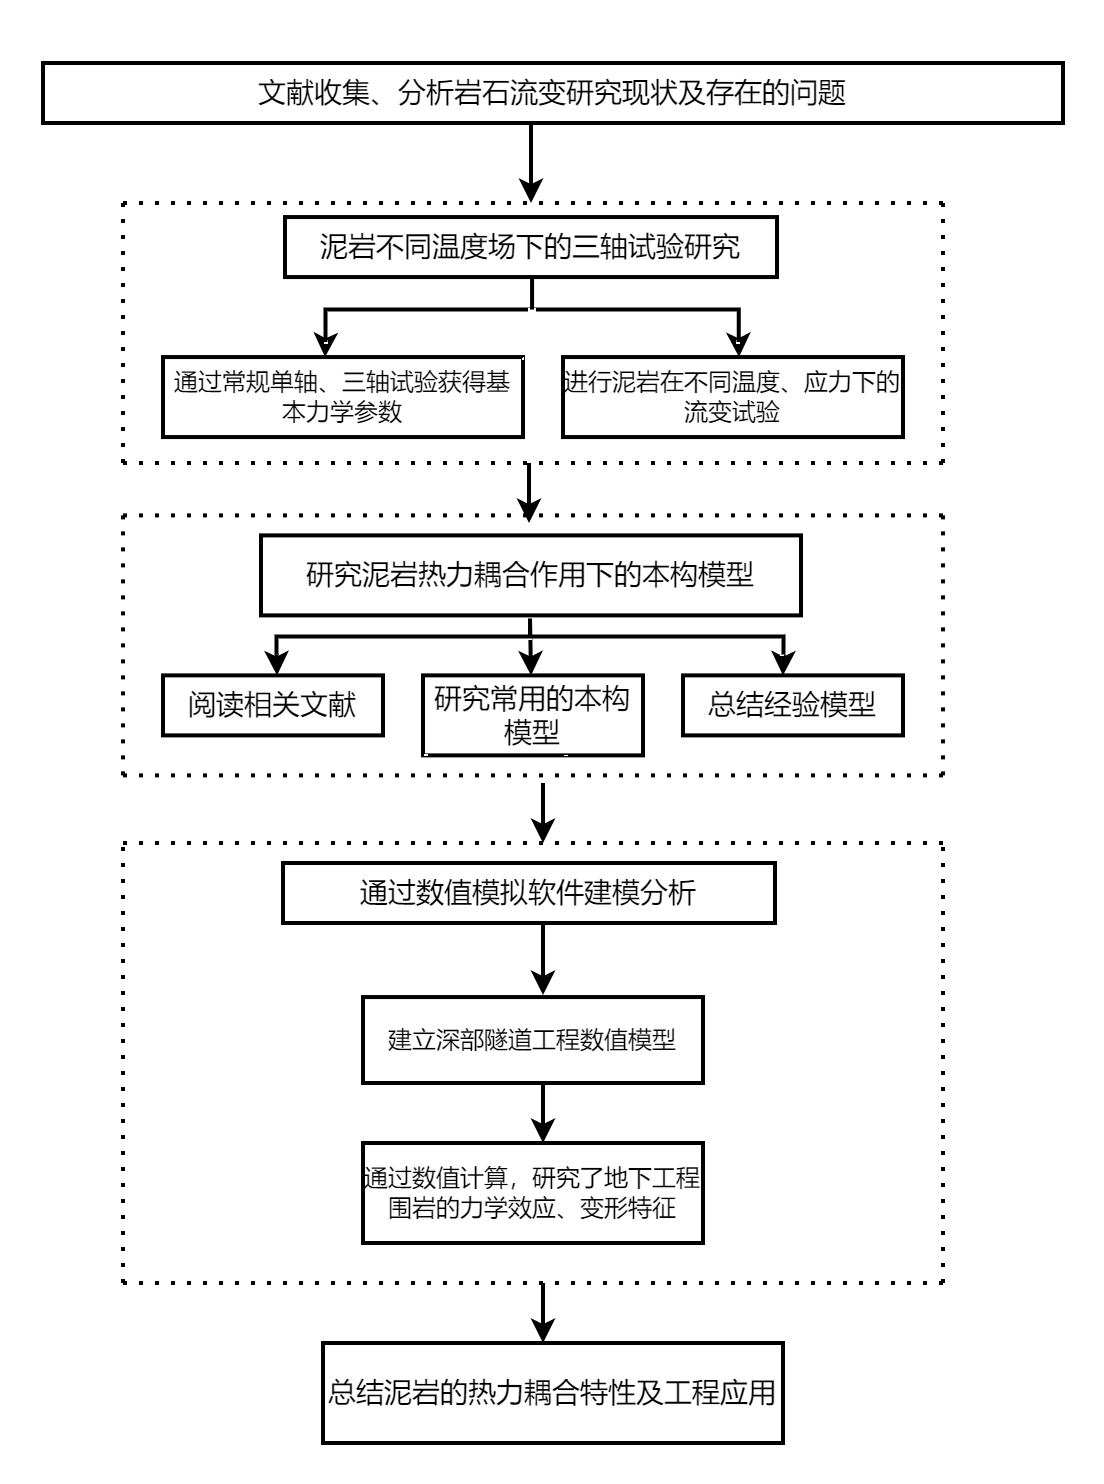
\includegraphics[width=0.9\textwidth]{img/chap1/技术路线.png}
    \caption{技术路线图}
    \label{fig:1-1}
\end{figure}


\section{主要创新点}

1.在单、三轴流变试验的基础上,考虑温度因素,进行热力耦合流变试验。首先进行泥岩的单、三轴压缩试验,根据泥岩的抗压强度确定进行流变试验时施加的轴向应力。在实际工程中需要考虑温度对岩石流变的影响,故温度试验是不可缺少的;

2.参考现有的模型,将温度的影响因子加入到本构模型中。考虑温度变化对流变过程的影响,通过试验数据拟合热力耦合作用下本构模型的参数;

3. 依托工程实际建立深部隧道工程的数值仿真模型。以新的本构模型为依据,对建立的模型进行不同温度下的流变过程模拟计算,并将模拟结果与试验获得的结论进行对比分析,验证本构模型的合理性。


\section{小结}

关于泥岩的热力耦合流变特性,查到的相关资料比较少,说明对泥岩热力耦合特性的研究成果较少






